\documentclass[12pt,aspectratio=169]{beamer}

\usetheme[progressbar=frametitle, numbering=fraction]{metropolis}
\usepackage{appendixnumberbeamer}
\usepackage{gensymb}
\usepackage{booktabs}
\usepackage[scale=2]{ccicons}

\usepackage{pgfplots}
\usepgfplotslibrary{dateplot}
% \usepackage[english]{babel}
\usepackage{babel}

\usepackage{xspace}
\newcommand{\themename}{\textbf{\textsc{metropolis}}\xspace}

% Chinese Fonts (Fontset: fandol,ubuntu)
\usepackage[fontset=windows]{ctex}

% Math Fonts
\usefonttheme{professionalfonts} 
\usepackage{mathspec}
\setsansfont[BoldFont={Fira Sans},
Numbers={OldStyle}]{Fira Sans Light}
\setmathsfont(Digits)[Numbers={Lining, Proportional}]{Fira Sans Light}

% Change Color of the theme
\usepackage{xcolor}
\definecolor{DarkGrey}{HTML}{353535}
\definecolor{ECNURed}{RGB}{164,31,53}
\definecolor{ECNUBrown}{RGB}{134,117,77}
\definecolor{BackGround}{RGB}{250,250,250}
\definecolor{MyBlue}{RGB}{0,161,233}
\definecolor{MyRed}{RGB}{228,0,127}
\setbeamercolor{normal text}{ fg= DarkGrey  }
\setbeamercolor{alerted text}{ fg= ECNURed  }
\setbeamercolor{example text}{ fg= ECNUBrown  }

% Bolder Fonts for presenting in a large room 
\setsansfont[BoldFont={Fira Sans SemiBold}]{Fira Sans}
\metroset{block=fill}

\usepackage{listings,xcolor}
\usepackage{tikz}
\usepackage{pgfmath}
\usepackage{animate,media9,graphicx}
\usepackage{calligra}
\usepackage{array}
\renewcommand{\arraystretch}{2}  % 增加行高
\setlength{\tabcolsep}{10pt}       % 增加列间距

\usepackage[backend=biber,style=gb7714-2015,sorting=none]{biblatex}
\setbeamerfont{bibliography item}{size=\footnotesize}
\setbeamerfont{bibliography entry author}{size=\footnotesize}
\setbeamerfont{bibliography entry title}{size=\footnotesize}
\setbeamerfont{bibliography entry location}{size=\footnotesize}
\setbeamerfont{bibliography entry note}{size=\footnotesize}
\renewcommand{\bibfont}{\footnotesize}
\addbibresource{slides.bib}

\lstset{
	language         = c++,
	numbers          = left,
	numberstyle      = \tiny,
	breaklines       = true,
	captionpos       = b,
	tabsize          = 4,
	frame            = shadowbox,
	columns          = fullflexible,
	commentstyle     = \color[RGB]{0,128,0},
	keywordstyle     = \color[RGB]{0,0,255},
	basicstyle       = \tiny\ttfamily,
	stringstyle      = \color[RGB]{148,0,209}\ttfamily,
	rulesepcolor     = \color{red!20!green!20!blue!20},
	showstringspaces = false,
}

\title{Mathematical Model of Servo Valve}
% \subtitle{}
\author{汇报人:丁逸飞}
\date{\today}
% \institute{}
% \titlegraphic{\hfill
\includegraphics[height=1.5cm]{ECNUlogo.png}}

\begin{document}

\maketitle
\footnotesize
% \begin{frame}{Contents}
%   \setbeamertemplate{section in toc}[sections numbered]
%   \tableofcontents%[hideallsubsections]
% \end{frame}

\begin{frame}{伺服阀结构图}

  \begin{figure}
    \begin{center}
      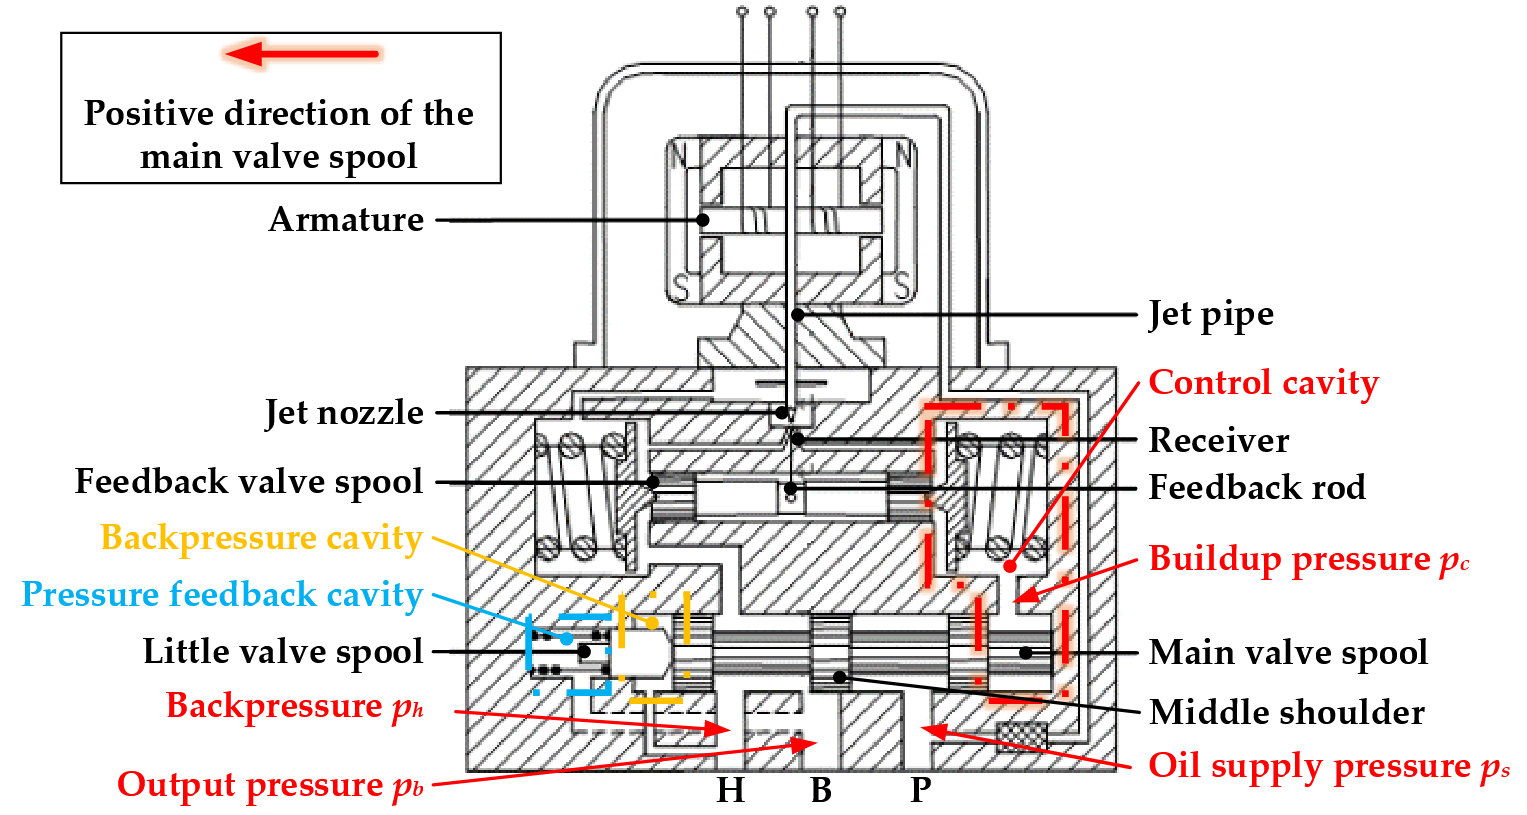
\includegraphics[width=0.85\textwidth]{fig/structure.png}
    \end{center}
    \caption{伺服阀结构图\cite{huang2022analysis}}\label{fig:1}
  \end{figure}

\end{frame}

\begin{frame}{工作压力和电流}

  \[
    \frac{P}{I}(s)=K\left[\frac{\omega_n^2}{\omega_n^2+2\zeta\omega_ns+s^2}\right]\text{\cite{matos2022aircraft}}
  \]

  $K:=$ pressure control servovalve static gain (压力控制伺服阀静态增益)

  $\omega_n=2\pi f_n:=$ apparent natural frequency (表观固有频率)

  $\zeta:=$ apparent damping ratio (表观阻尼比)

  $P:=$ servovalve differential pressure output (伺服阀压差输出,即\textbf{\color{ECNURed}工作压力})

  $I:=$ differential current input to servovalve (伺服阀的差分\textbf{\color{ECNURed}电流}输入)

  $s:=$ Laplace operator

  拉普拉斯逆变换后:$\displaystyle\frac{\textrm{d}^2P(t)}{\textrm{d}t^2}+2\zeta\omega_n
  \frac{\textrm{d}P(t)}{\textrm{d}t}+\omega_n^2P(t)=K\omega_n^2I(t)$

\end{frame}

\begin{frame}{References}
  
  \printbibliography[heading=none]

\end{frame}

\begin{frame}{Acknowledgement}

  \begin{center}

    \textcolor{gray}{\Huge{\centerline{\calligra{Thank you!}}}}

  \end{center}

\end{frame}

\end{document}
